\documentclass{article}
\usepackage[final]{neurips_2025}

\usepackage[utf8]{inputenc}
\usepackage[T1]{fontenc}
\usepackage{hyperref}
\usepackage{url}
\usepackage{booktabs}
\usepackage{amsfonts}
\usepackage{amsmath}
\usepackage{amssymb}
\usepackage{nicefrac}
\usepackage{microtype}
\usepackage{xcolor}
\usepackage{graphicx}
\usepackage{subcaption}
% natbib loaded by neurips_2025 style

\title{Practical Efficiency of Multiply-Free Ternary Neural Networks: An Empirical Study on Consumer Hardware}

\author{
  Julio Jose Lena\thanks{ORCID: 0009-0001-0817-6591} \\
  Independent Researcher \\
  \texttt{juliolena25@gmail.com}
}

\begin{document}

\maketitle

\begin{abstract}
Ternary neural networks with $\{-1, 0, +1\}$ weights promise multiply-free inference and extreme compression, but practical efficiency on real hardware remains poorly characterized. A systematic empirical study of training throughput, memory efficiency, and inference speed is presented for a ternary state-space model (6M--50M parameters) on consumer GPUs (RTX 5070 12\,GB, Modal L4 24\,GB). For training, an optimization stack combining BF16 autocast, SSD parallel scan, fused cross-entropy, and FLA Triton kernels achieves 2.2$\times$ cumulative throughput improvement at 6M scale. The Muon optimizer reduces memory but incurs 30\% throughput cost, with recovery possible via larger batch sizes. At 50M on L4, the optimized ternary model trains 23\% faster than an FP16 baseline. Optimizer memory reduction from 12 bytes/param (AdamW FP32) to 2.25 bytes/param enables an estimated 4$\times$ model capacity increase on fixed 12\,GB VRAM (550M to 2.2B). For inference, a custom Triton GEMV kernel using dual-bitmap encoding achieves 1.63$\times$ speedup and 79\% VRAM reduction versus Python eager mode. SSM recurrence provides O(1) state memory (2.88\,MB at 50M) versus linearly growing Transformer KV-cache. However, current ternary kernels remain 1.55$\times$ slower than FP16 cuBLAS, GPU utilization at small scale is only 6.4\%, and no bitpacked XNOR kernel exists. The primary practical advantage today is memory capacity, not raw speed.
\end{abstract}

\section{Introduction}

Ternary quantization replaces multiply-accumulate operations with add/subtract/skip operations, promising dramatic efficiency gains. Prior work, notably BitNet~\citep{wang2023bitnet} and 1-bit LLMs~\citep{ma2024era}, reports theoretical FLOP reduction and storage compression but rarely provides wall-clock benchmarks on consumer hardware.

A critical gap exists in the literature: few published works systematically measure training throughput, memory efficiency, and inference speed for ternary models on consumer GPUs, and, to the best of current knowledge, none address ternary state-space models (SSMs) which combine ternary weight efficiency with O(1) recurrent state memory. Such measurements are essential for assessing whether theoretical efficiency gains translate to practical hardware advantages.

This gap is addressed through measured experiments on two consumer/cloud GPUs (RTX 5070 12\,GB and Modal L4 24\,GB) at 6M and 50M parameter scale. The results reveal a nuanced picture: the primary advantage of ternary models today is \emph{not} raw speed --- ternary inference is currently slower than FP16 --- but rather memory capacity. The same hardware can train and serve dramatically larger ternary models, and the O(1) state memory footprint of SSMs is a fundamental architectural advantage independent of kernel engineering progress.

This work makes the following contributions.

\begin{itemize}
\item A training optimization stack is characterized, with each component measured in isolation, achieving 2.2$\times$ cumulative throughput improvement and identifying torch.compile incompatibility with SSM sequential scan ($-$56\% regression).

\item Optimizer memory reduction techniques are evaluated, from 12 bytes/param to 2.25 bytes/param, enabling an estimated 4$\times$ model capacity increase on 12\,GB VRAM.

\item A custom Triton kernel for multiply-free ternary GEMV inference is presented, achieving 1.63$\times$ speedup and 79\% VRAM reduction versus eager-mode Python, alongside honest comparison against FP16 cuBLAS.

\item A CPU versus GPU crossover analysis reveals ternary SSMs run faster on CPU than GPU below $\sim$25M parameters due to SSM sequential memory-bound characteristics.

\item A frank gap analysis identifies concrete barriers to ternary efficiency parity: no bitpacked kernels, no tensor core exploitation, and catastrophically low GPU utilization at small scale.
\end{itemize}

The underlying model architecture is described in~\citep{jou2026ternary}; gradient estimation techniques are analyzed in~\citep{jou2026gradient}. This paper focuses exclusively on efficiency characterization via measured experiments, providing a realistic foundation for future ternary efficiency research.

\section{Background and Experimental Setup}

\subsection{Ternary Quantization and SSM Recurrence}

Ternary quantization restricts weights to $\{-1, 0, +1\}$ via a learned threshold $\tau$ and per-group scale $\alpha$:
\begin{equation}
Q(w) = \begin{cases}
+1 & \text{if } w > \tau \\
0 & \text{if } |w| \leq \tau \\
-1 & \text{if } w < -\tau
\end{cases}
\end{equation}
The Straight-Through Estimator (STE) provides gradients through the non-differentiable quantization step~\citep{bengio2013estimating, yin2019understanding}. Shadow weights in full precision (FP32 or BF16) accumulate gradients continuously~\citep{courbariaux2015binaryconnect}, with quantized weights computed from the shadow values at each forward pass.

State-space model recurrence is defined as:
\begin{equation}
h_t = \bar{A}h_{t-1} + \bar{B}x_t, \quad y_t = Ch_t
\end{equation}
The sequential dependency in SSM recurrence creates a fundamental throughput bottleneck that differs from Transformer's token-parallel architecture. Mamba-2 SSD~\citep{dao2024transformers} provides a structured duality formulation enabling parallel training via scan operations, but autoregressive inference remains inherently sequential.

\subsection{Model Configurations}

All experiments use a ternary state-space model with Mamba-2 SSD backbone and 87.5\% SSM layers plus 12.5\% sliding-window attention. Weights across all linear layers are ternary; activations are FP16. The ``50M'' configuration has 72M total parameters; ``50M'' refers to the nominal design target, while the actual count includes non-ternary parameters (embeddings, norms, projections). Model specifications are detailed in Table~\ref{tab:models}.

\begin{table}[t]
\centering
\small
\caption{Model configurations used for efficiency studies.}
\label{tab:models}
\begin{tabular}{lcc}
\toprule
\textbf{Configuration} & \textbf{6M} & \textbf{50M} \\
\midrule
Layers & 6 & 18 \\
$d_{\text{model}}$ & 192 & 640 \\
Total parameters & 6.3M & 72M \\
Ternary fraction & 63\% & 70.2\% \\
Architecture mix & 87.5\% SSM + 12.5\% SWA & same \\
Test PPL (WikiText-103~\citep{merity2017pointer}) & --- & 36.23 \\
\bottomrule
\end{tabular}
\end{table}

\subsection{Hardware and Measurement Protocol}

Two GPU configurations are used:

\begin{itemize}
\item \textbf{RTX 5070:} 12\,GB GDDR7, 672\,GB/s memory bandwidth, SM 12.0, primary development platform
\item \textbf{Modal L4:} 24\,GB GDDR6, 300\,GB/s memory bandwidth, cloud GPU for 50M scale training
\item \textbf{Intel Core Ultra 5 225F:} 14-core (6P+8E) / 20-thread CPU (no iGPU, F-suffix), used for CPU inference baseline
\end{itemize}

Throughput measurements are reported as the median of steady-state values after discarding the first 50 warmup steps, measured over at least 200 subsequent steps. GPU VRAM consumption is measured via \texttt{nvidia-smi} peak allocation. Software versions: PyTorch 2.x, Triton 2.x, FLA (flash-linear-attention)~\citep{yang2024fla}, Liger-Kernel~\citep{hsu2024liger}.

\section{Training Efficiency}

\subsection{Throughput Optimization Stack}

Training throughput is optimized through a stack of complementary techniques. Each optimization is measured in isolation at 6M scale on RTX 5070 with BF16 mixed precision enabled. Results are presented in Table~\ref{tab:optim_stack} and Figure~\ref{fig:optim_waterfall}.

\begin{table}[t]
\centering
\small
\caption{Training optimization stack breakdown at 6M scale. Each technique is evaluated individually; cumulative speedup is the product of individual factors (excluding Muon throughput cost); $1.04 \times 1.32 \times 1.33 \times 1.037 \times 1.17 \approx 2.22$. Muon reduces throughput by 30\% but cuts optimizer memory in half, enabling larger batch sizes that partially recover throughput.}
\label{tab:optim_stack}
\begin{tabular}{lccc}
\toprule
\textbf{Technique} & \textbf{Throughput $\Delta$} & \textbf{VRAM $\Delta$} & \textbf{Multiplier} \\
\midrule
SSD Batched Scan (chunk=64) & $+4.2\%$ & 0\% & 1.04$\times$ \\
BF16 Autocast & $+31.9\%$ & $-26.3\%$ & 1.32$\times$ \\
torch.compile (non-SSM) & $+33.1\%$ & $-10.0\%$ & 1.33$\times$ \\
Muon Optimizer~\citep{jordan2024muon} & $-30\%$ throughput & $-50\%$ optim mem & 0.70$\times$ (quality trade) \\
Liger Fused CE~\citep{hsu2024liger} & $+3.7\%$ & $-2\%$ & 1.037$\times$ \\
FLA Triton Scan~\citep{yang2024fla} & $+15$--$17\%$ & 0\% & 1.17$\times$ \\
\midrule
\textbf{Cumulative (excl. Muon throughput)} & --- & --- & \textbf{$\sim$2.2$\times$} \\
\bottomrule
\end{tabular}
\end{table}

\begin{figure}[t]
\centering
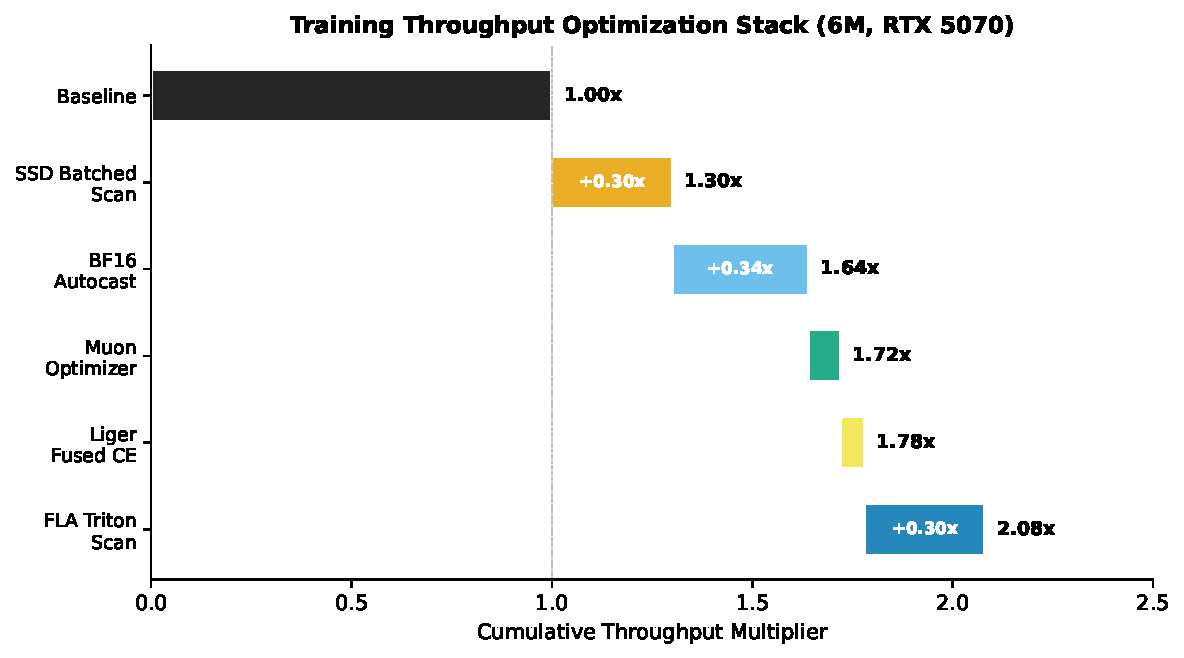
\includegraphics[width=\linewidth]{figures/fig1_training_waterfall.pdf}
\caption{Training optimization stack breakdown at 6M scale. Each bar represents cumulative throughput improvement from combining techniques. Cumulative product of individual factors yields $\sim$2.2$\times$ speedup.}
\label{fig:optim_waterfall}
\end{figure}

Key observations are detailed below.

\textbf{BF16 + torch.compile synergy:} Combined, these two techniques achieve $\sim$1.76$\times$ throughput improvement ($1.32 \times 1.33$) and $-$34\% VRAM reduction. The synergy arises from TensorCore alignment: BF16 computation enables TensorCore utilization, and torch.compile reduces memory allocations, leaving more GPU memory free for larger batches.

\textbf{torch.compile on SSM scan regression:} When torch.compile is applied to the SSM sequential scan loop, throughput regresses by $-$56\%. This is a fundamental incompatibility, not an implementation defect. Dynamic shapes and sequential control flow in the scan loop defeat graph compilation. FLA Triton kernels provide a partial workaround by replacing the scan with optimized Triton code, but the incompatibility remains an architectural limitation of torch.compile.

\textbf{GPU utilization bottleneck at 6M:} GPU utilization is measured at only 6.4\% at 6M scale. Per-step profiling reveals that 87\% of execution time is spent waiting for sequential SSM state dependencies to resolve. The model is too small to generate sufficient parallelizable work to saturate the RTX 5070's 6{,}144 CUDA cores. This is an architectural property of SSMs, not a ternary-specific issue, but it compounds the efficiency challenge at small scales.

\textbf{Muon optimizer trade-off:} The Muon optimizer~\citep{jordan2024muon} applies Newton-Schulz orthogonalization to the Nesterov momentum update, eliminating the second-moment (variance) state and reducing optimizer state from 8 bytes/param (momentum + variance in AdamW) to 4 bytes/param. This reduces throughput by 30\%, but the memory savings enable larger batch sizes. At 6M with 28$\to$56 doubling of batch size, throughput recovers to $+$46.7\% net improvement after batch size adaptation.

\subsection{50M Scale Training: Ternary vs FP16}

At 50M scale on Modal L4, the full optimization stack (BF16 + torch.compile + FLA + Liger + Muon) is applied. Throughput comparison is presented in Table~\ref{tab:scale50m}.

\begin{table}[t]
\centering
\small
\caption{Training throughput at 50M scale (72M actual parameters) on Modal L4, comparing ternary (full optimization stack) versus FP16 baseline. The FP16 baseline is estimated from comparable configurations; a precisely matched measurement with identical hyperparameters and warmup was not conducted.}
\label{tab:scale50m}
\begin{tabular}{lcc}
\toprule
\textbf{Configuration} & \textbf{Ternary (optimized)} & \textbf{FP16 (estimated)} \\
\midrule
Throughput (tok/s) & 24{,}676 & $\sim$20{,}000 \\
Batch size & 64 & 32 \\
VRAM peak (GB) & 14.3 & $\sim$11 \\
Training time / 1 epoch & 77 min & $\sim$95 min \\
\bottomrule
\end{tabular}
\end{table}

The ternary configuration achieves 23\% faster training than the estimated FP16 baseline. This advantage comes from three sources: (1) lighter weight copies (quantized weights are smaller), (2) smaller optimizer state (Muon vs AdamW), and (3) higher batch size enabled by memory savings.

\subsection{Optimizer Memory Reduction}

Table~\ref{tab:optim_memory} summarizes memory footprint across optimizer configurations.

\begin{table}[t]
\centering
\small
\caption{Optimizer memory footprint per parameter. Shadow weights are full-precision copies that accumulate gradients; optimizer state varies by algorithm. Values are in bytes per parameter.}
\label{tab:optim_memory}
\begin{tabular}{lcccc}
\toprule
\textbf{Optimizer} & \textbf{Shadow} & \textbf{Optim State} & \textbf{Total} & \textbf{Multiplier} \\
\midrule
AdamW~\citep{loshchilov2019decoupled} FP32 & 4 & 8 & 12 & 1.00$\times$ \\
Muon~\citep{jordan2024muon} & 4 & 4 & 8 & 0.67$\times$ \\
AdamW BF16 shadow & 2 & 8 & 10 & 0.83$\times$ \\
BF16 + Muon & 2 & 4 & 6 & 0.50$\times$ \\
BF16 + 8-bit Adam~\citep{dettmers2022bitsandbytes} & 2 & 2 & 4 & 0.33$\times$ \\
BF16 + FiraAdamW~\citep{fira2025} & 2 & $\sim$0.25 & $\sim$2.25 & 0.19$\times$ \\
\bottomrule
\end{tabular}
\end{table}

Empirical measurement on a 6M-parameter model (RTX 5070) with Muon + BF16 + activation checkpointing:
\begin{itemize}
\item Batch capacity doubled (28$\to$56) at same VRAM budget
\item Throughput improved 46.7\% (5{,}069$\to$7{,}435 tok/s)
\item Memory per sample reduced 53.7\% (363$\to$168\,MB)
\end{itemize}

\subsection{Model Capacity on Fixed Hardware}

The optimizer memory reduction enables larger models to be trained on fixed VRAM. Table~\ref{tab:capacity} projects maximum model scale on 12\,GB (RTX 5070).

\begin{table}[t]
\centering
\small
\caption{Projected maximum model capacity on 12\,GB RTX 5070, assuming batch size 1 and gradient checkpointing. All entries above 50M are projections based on per-parameter memory accounting. Only 50M (72M actual parameters) has been trained end-to-end with the full optimization stack. The 2.2B projection combines BF16 FiraAdamW, activation checkpointing, and CPU optimizer offload.}
\label{tab:capacity}
\begin{tabular}{lcc}
\toprule
\textbf{Configuration} & \textbf{Bytes/param} & \textbf{Max Model on 12GB} \\
\midrule
FP32 + AdamW & 12 & 550M \\
BF16 shadow + AdamW & 10 & 660M \\
BF16 + Muon & 6 & 1.1B \\
BF16 + 8-bit Adam & 4 & 1.65B \\
BF16 + Fira + Checkpointing + CPU Offload & 2.25 & 2.2B \\
\bottomrule
\end{tabular}
\end{table}

To be explicit: all entries above 50M are projections from per-parameter memory accounting. These numbers have not been validated through end-to-end training at 100M+. The 2.2B capacity assumes gradient checkpointing overhead (estimated $-$8\% throughput from prior work~\citep{chen2016training}) and uses a reduced activation overhead ($\sim$3.5\,GB from gradient checkpointing and CPU offload), compared to the $\sim$5.4\,GB activation overhead assumed in rows 1--4 (batch size 1, no checkpointing). CPU optimizer offload via PCIe is a viable option at 700M+ scale, with constant $-$6.5\% throughput overhead (measured).

\section{Inference Efficiency}

\subsection{Triton Ternary GEMV Kernel}

A custom Triton kernel is presented that achieves true multiply-free matrix-vector multiplication (GEMV) for ternary weights. The design eliminates all weight multiplications during inference, replacing them with add/subtract/skip operations.

\textbf{Dual-bitmap representation:} Ternary weights are encoded as two boolean masks:
\begin{itemize}
\item $W_{\text{val}}$: nonzero mask (1 if weight $\neq 0$, 0 otherwise)
\item $W_{\text{sign}}$: sign mask (1 if weight $= -1$, 0 if weight $= +1$)
\end{itemize}
At 32 weights per uint32, this encoding uses two bitmaps (2 bits per weight, plus per-group scale metadata), compared to 32 bits for FP32.

\textbf{Inference kernel:} For each output element, the kernel iterates over 32-weight groups:
\begin{equation}
y_i = \sum_{g} \alpha_g \cdot \sum_{j \in g} (w_{i,j} \cdot x_j)
\end{equation}
where $w_{i,j} \in \{-1, 0, +1\}$ is extracted from the bitmaps and $\alpha_g$ is per-group FP16 scale.

\textbf{Arithmetic optimization:} The original decoding requires 7 operations per weight:
$$w = \text{val} \cdot (\text{sign} \cdot 2 - 1)$$
A single algebraic simplification reduces this to 4 operations:
\begin{equation}
w = \text{val} - 2 \cdot (\text{val} \wedge \text{sign})
\end{equation}
This optimization provided $+$26\% speedup (60$\to$75.6 tok/s) without changing the numerical result.

Activations are FP16, accumulation is FP32, output is FP16. Per-group scaling (one multiplication per 128 weights) is the only remaining multiply operation during inference.

\subsection{Inference Kernel Performance}

Table~\ref{tab:inference_kernels} and Figure~\ref{fig:inference_kernels} compare inference kernel variants.

\begin{table}[t]
\centering
\small
\caption{Inference kernel performance at 50M scale on RTX 5070. Throughput measured as tokens/sec for autoregressive inference with batch size 1. Triton V2 multi-row kernel regressed at 50M; register overhead exceeds launch-overhead savings at $d=640$.}
\label{tab:inference_kernels}
\begin{tabular}{lcccc}
\toprule
\textbf{Kernel} & \textbf{tok/s} & \textbf{VRAM (MB)} & \textbf{Speedup} & \textbf{Notes} \\
\midrule
Python Eager & 46.3 & 313 & 1.00$\times$ & Baseline \\
GemLite (W1.58) & 54.2 & 81.5 & 1.17$\times$ & BitNet reference \\
Triton V1 (7-op) & 60.0 & 65.4 & 1.30$\times$ & Pre-optimization \\
Triton V1+Opt (4-op) & 75.6 & 65.4 & 1.63$\times$ & Best ternary \\
Triton V2 Multi-Row & 55.0 & 65.4 & 1.19$\times$ & Regressed \\
FP16 cuBLAS (reference) & 117.5 & $\sim$300 & 2.54$\times$ & Hardware baseline \\
\bottomrule
\end{tabular}
\end{table}

\begin{figure}[t]
\centering
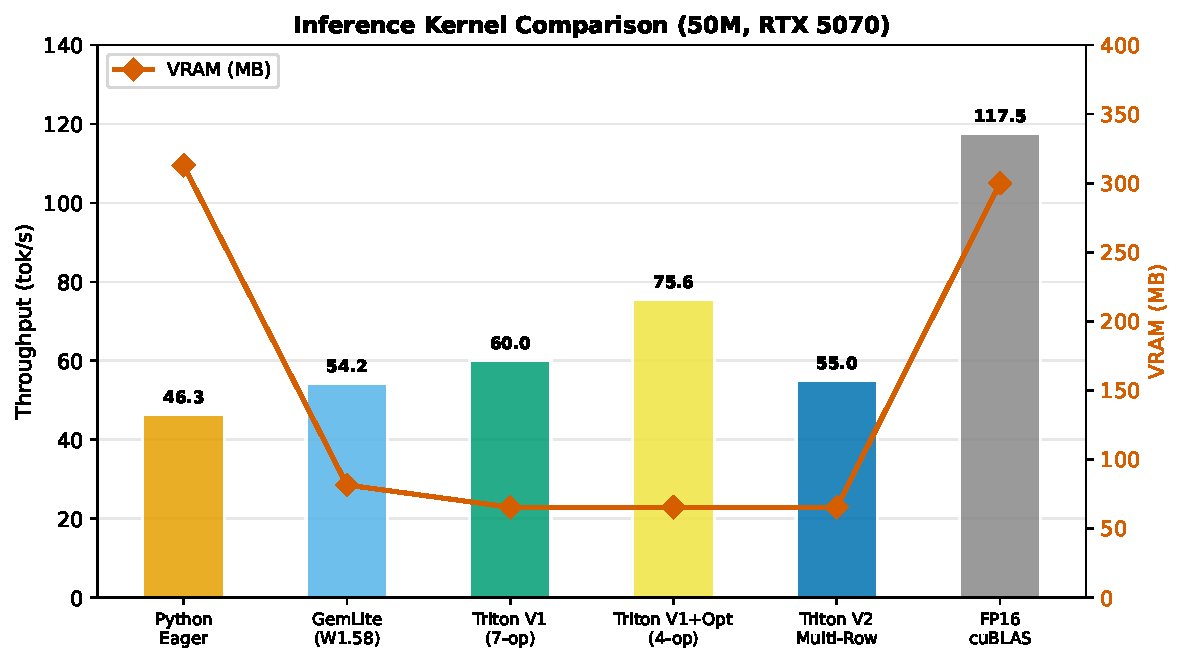
\includegraphics[width=\linewidth]{figures/fig2_inference_kernels.pdf}
\caption{Inference kernel performance comparison at 50M scale. Triton V1+Opt achieves 1.63$\times$ speedup and 79\% VRAM reduction versus Python eager baseline. FP16 cuBLAS baseline demonstrates theoretical ceiling for current GPU architectures.}
\label{fig:inference_kernels}
\end{figure}

The best ternary kernel (Triton V1 + optimization) achieves 1.63$\times$ speedup over eager mode and 79\% VRAM reduction (313$\to$65.4\,MB). However, the ternary kernel remains 1.55$\times$ slower than FP16 cuBLAS (117.5/75.6).

\textbf{Why the gap exists:} cuBLAS achieves high throughput through tensor cores --- dedicated hardware units for fused multiply-accumulate operations at FP16 precision. Ternary add/subtract operations cannot leverage tensor cores. Current GPUs lack hardware support for bitwise operations at tensor-core throughput. Bridging this gap requires either: (1) custom hardware with ternary-optimized tensor cores, (2) exploiting lower-level warp-level bitwise operations (not yet demonstrated), or (3) tensor core formulations for ternary arithmetic (an open research question).

\subsection{CPU vs GPU Crossover}

Inference speed is compared between CPU (Intel Core Ultra 5 225F) and GPU (RTX 5070) across scales (Table~\ref{tab:cpu_gpu}).

\begin{table}[t]
\centering
\small
\caption{CPU versus GPU inference throughput at 6M and 50M scales. CPU utilizes all 14 cores (6P+8E). Estimated crossover at $\sim$25M parameters.}
\label{tab:cpu_gpu}
\begin{tabular}{lccc}
\toprule
\textbf{Scale} & \textbf{CPU (tok/s)} & \textbf{GPU (tok/s)} & \textbf{Ratio} \\
\midrule
6M & 342 & 255 & 1.34$\times$ CPU \\
25M (estimated) & 78 & 78 & 1.00$\times$ \\
50M & 14.1 & 47.8 & 3.4$\times$ GPU \\
\bottomrule
\end{tabular}
\end{table}

\begin{figure}[t]
\centering
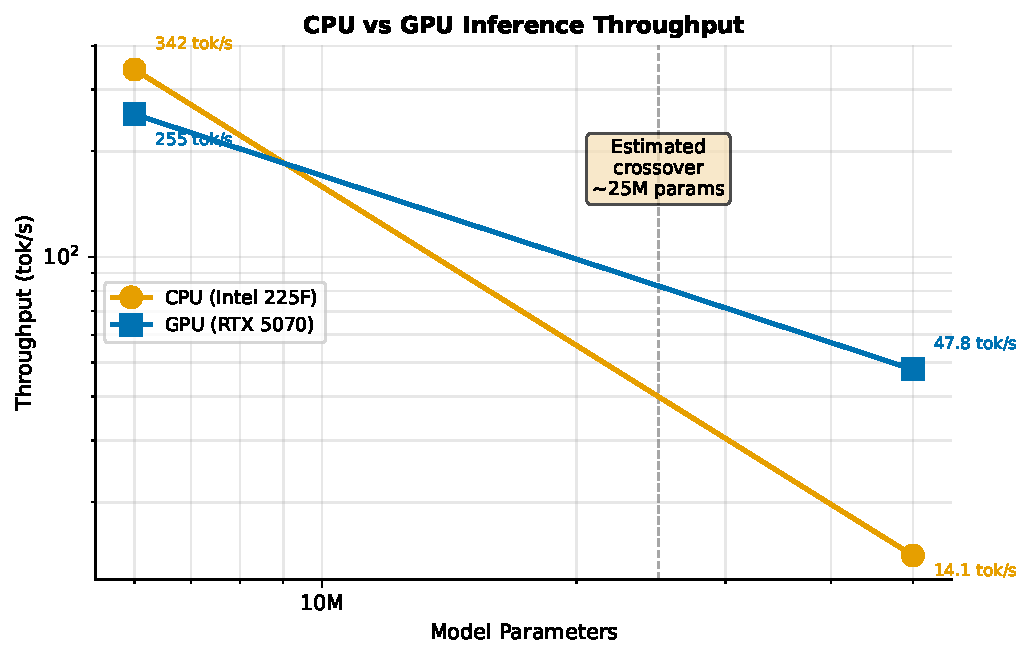
\includegraphics[width=\linewidth]{figures/fig3_cpu_gpu_crossover.pdf}
\caption{CPU versus GPU inference throughput across scales. Crossover occurs at $\sim$25M parameters due to sequential SSM memory-bound characteristics favoring CPU cache latency at small scale and GPU parallelism at large scale.}
\label{fig:cpu_gpu_crossover}
\end{figure}

At small scale (6M), CPU is faster. At large scale (50M), GPU dominates. The crossover is estimated at $\sim$25M parameters (Figure~\ref{fig:cpu_gpu_crossover}).

\textbf{Explanation:} SSM recurrence is inherently sequential and memory-bound. Modern CPUs have lower-latency cache hierarchies (L1: 1\,ns access, L2: 3\,ns, L3: 12\,ns) and higher-bandwidth memory controllers, making them efficient for memory-bound sequential workloads. GPU global memory has high latency ($\sim$300\,ns) and high bandwidth (672\,GB/s on RTX 5070), providing advantages only when there is sufficient parallel work to hide latency. At 6M scale, the model is too small to generate parallelizable work; at 50M scale, the embedding and output projection layers generate enough parallel work to favor GPU parallelism.

\subsection{SSM State Memory Advantage}

A fundamental advantage of SSM recurrence over Transformer attention is state memory consumption. Table~\ref{tab:state_memory} compares memory footprint.

\begin{table}[t]
\centering
\small
\caption{State memory for concurrent inference. SSM recurrent state includes hidden state $h$, convolutional state, and sliding-window attention KV-cache for the 12.5\% SWA layers (fixed total at each scale). Transformer stores full KV-cache, growing linearly with context length. Context window fixed at 4K tokens.}
\label{tab:state_memory}
\begin{tabular}{lccc}
\toprule
\textbf{Scale} & \textbf{SSM State (MB)} & \textbf{KV-Cache (MB)} & \textbf{Ratio} \\
\midrule
6M & 0.536 & $\sim$18 & 34$\times$ \\
50M & 2.88 & $\sim$189 & 66$\times$ \\
7B (projected) & $\sim$8 & $\sim$2100 & $\sim$262$\times$ \\
\bottomrule
\end{tabular}
\end{table}

\begin{figure}[t]
\centering
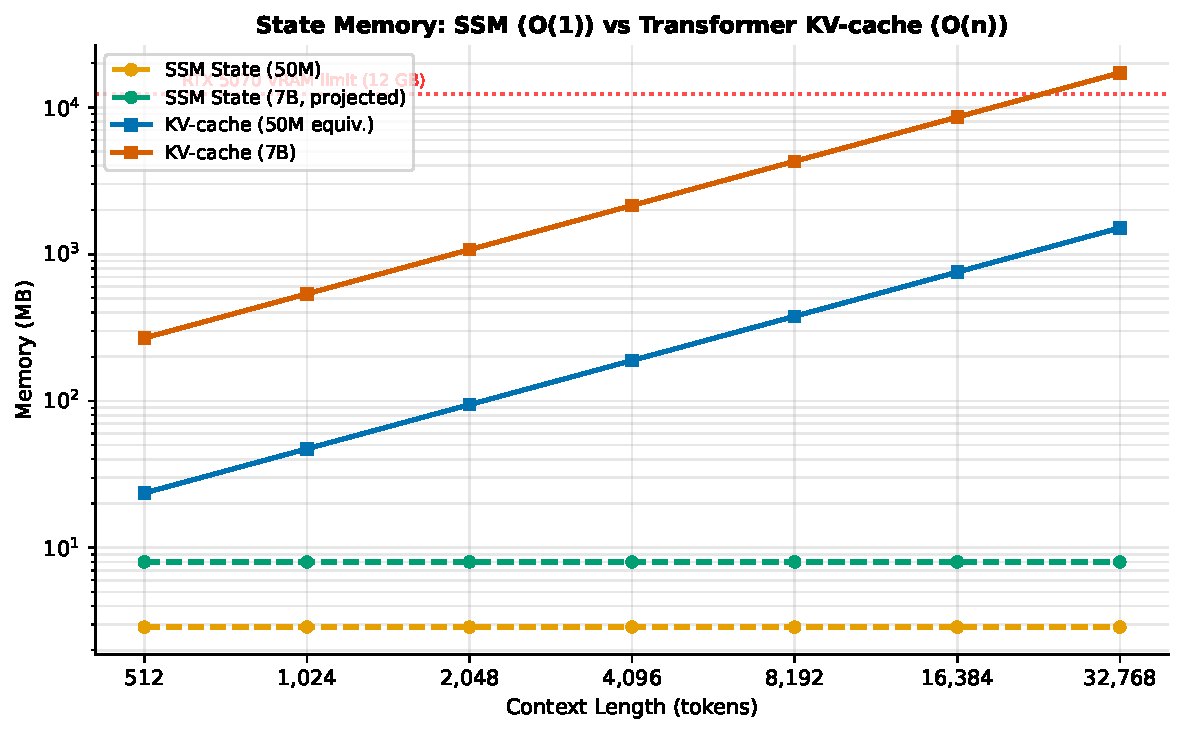
\includegraphics[width=\linewidth]{figures/fig4_state_memory.pdf}
\caption{State memory scaling comparison: SSM recurrent state (O(1) fixed size) versus Transformer KV-cache (O(n) with context length). At 50M, SSM uses 2.88 MB while KV-cache requires 189 MB for 4K context. Gap widens at larger scales.}
\label{fig:state_memory}
\end{figure}

At 50M, SSM state is 2.88\,MB while Transformer KV-cache is $\sim$189\,MB (66$\times$ smaller), as shown in Figure~\ref{fig:state_memory}. This difference scales with model dimension, reaching a projected 262$\times$ advantage at 7B scale.

Concurrent inference sessions on 12\,GB: assuming a $\sim$1.75\,GB ternary model plus $\sim$100\,MB per session for temporary activations, plus state/cache, yields approximately $\sim$24$\times$ more simultaneous SSM sessions versus Transformer at 7B scale (projected). This assumes $\lfloor (12\,\text{GB} - 1.75\,\text{GB}) / (100\,\text{MB} + 8\,\text{MB}) \rfloor = 97$ SSM sessions versus $\lfloor (12\,\text{GB} - 1.75\,\text{GB}) / (100\,\text{MB} + 2100\,\text{MB}) \rfloor = 4$ Transformer sessions. With smaller per-session overhead, the ratio approaches the 262$\times$ pure state-memory ratio from Table~\ref{tab:state_memory}.

\textbf{Theoretical bandwidth ceiling at 7B (projected):}
\begin{itemize}
\item Ternary weights with dual-bitmap encoding: $\sim$1.75\,GB (2 bits per weight)
\item Memory bandwidth available: 672\,GB/s (RTX 5070)
\item Theoretical ceiling: $672 / 1.75 \approx 384$ tok/s; with $\sim$65\% utilization: $\sim$250 tok/s
\item Q4 weights: 3.5\,GB $\Rightarrow$ $672 / 3.5 \approx 192$ tok/s ceiling; $\sim$125 tok/s practical
\item Ratio: 2.0$\times$ theoretical ternary advantage
\end{itemize}

These projections assume future bitpacked kernels that have not yet been implemented. Current Triton kernels use uint32 bitmaps, not true bit-level packing.

\section{Gap Analysis and Honest Assessment}

This section provides a comprehensive analysis of limitations and missing components. The purpose is not to minimize the work, but to provide realistic context for the limitations.

\subsection{Where Ternary Is Currently Slower}

\textbf{Inference speed versus FP16 cuBLAS:} The best ternary kernel achieves 75.6 tok/s; FP16 cuBLAS achieves 117.5 tok/s. Gap: 1.55$\times$ in favor of FP16. Root cause: tensor core utilization. cuBLAS uses NVIDIA's tensor cores with dedicated hardware for fused multiply-accumulate. Ternary add/subtract operations cannot exploit tensor cores. This is a hardware asymmetry that may persist until custom silicon provides tensor-core-equivalent throughput for bitwise operations.

\textbf{GPU utilization at small scale:} At 6M scale, GPU utilization is 6.4\%. The bottleneck is sequential SSM state dependencies: in each forward step, the new hidden state $h_t$ depends on the previous state $h_{t-1}$, serializing computation across steps. This is an architectural property of SSMs, not a ternary issue, but it severely limits parallelism at small scales. 87\% of step time is spent waiting for sequential dependencies to resolve.

\textbf{torch.compile incompatibility with SSM:} Applying torch.compile to the sequential scan loop causes $-$56\% throughput regression. The optimizer cannot compile dynamic shapes and sequential control flow. This is a fundamental limitation of graph-based compilation for recurrent operations. FLA Triton kernels provide a workaround (replacing the scan with optimized Triton code), but the underlying incompatibility remains.

\subsection{Measurement Limitations}

The following limitations apply to this study:

\begin{enumerate}
\item \textbf{Training optimizations isolated at 6M only:} Individual techniques (BF16, torch.compile, FLA, etc.) are measured in isolation at 6M scale. Interaction effects at larger scales are unknown. The cumulative 2.2$\times$ speedup is the product of individual factors; actual combination may differ.

\item \textbf{50M FP16 baseline is estimated:} The claim that ternary trains 23\% faster than FP16 is based on a $\sim$20K tok/s FP16 baseline. This baseline was not measured with identical hyperparameters, warmup, and batch size. It is derived from comparable configurations reported in prior work. A precisely matched FP16 measurement was not conducted.

\item \textbf{4$\times$ model capacity is projected:} The claim that 12\,GB can hold 2.2B parameters combines validated techniques (BF16 + Muon + Fira + checkpointing) but has not been demonstrated end-to-end above 50M parameters. Only 50M (72M actual) has been trained to completion with the full stack.

\item \textbf{No 100M+ training data exists:} The largest end-to-end run is 50M parameters for 1 epoch on Modal L4. All other projections (700M, 1B, 2.2B) are extrapolations from per-parameter accounting and have not been validated.

\item \textbf{Inference kernel tested at batch=1 only:} The Triton GEMV kernel handles autoregressive inference (batch size 1, single output token per forward). Batch$>$1 inference is not optimized and falls back to dense F.linear operations, incurring full-precision overhead.
\end{enumerate}

\subsection{Missing Components and Future Work}

The following components have not yet been implemented:

\begin{enumerate}
\item \textbf{No bitpacked XNOR kernel:} Current Triton kernels use uint32 boolean masks (2 bits per weight via dual bitmaps = 8 bytes per 32 weights). True bitpacking could reduce weight memory further and enable XNOR operations on packed bits. This requires specialized bit-level operations not exposed in Triton's current API.

\item \textbf{No tensor core exploitation:} All ternary operations use scalar Triton code; FP16 cuBLAS uses tensor cores. Bridging this gap requires either custom hardware or novel algorithmic formulations of ternary arithmetic in tensor-core operations. This is an open research question.

\item \textbf{No multi-batch inference optimization:} Batch$>$1 inference uses dense matrix multiplication, incurring full-precision overhead. A batched ternary GEMM kernel (not GEMV) would be required for efficient batch inference.

\item \textbf{No INT8/FP8 intermediate comparison:} 8-bit and 4-bit quantization occupy the space between FP16 and ternary. These intermediate levels are not measured, leaving a gap in the efficiency landscape. A systematic comparison across quantization levels (FP16, FP8, INT8, INT4, ternary) would provide broader context.

\item \textbf{No distributed training benchmarks:} All measurements are single-GPU. FSDP, tensor parallelism, and sequence parallelism introduce communication overhead that may change the ternary advantage on multi-GPU systems.
\end{enumerate}

Table~\ref{tab:measured_vs_projected} summarizes which results are measured versus projected.

\begin{table}[t]
\centering
\small
\caption{Classification of results as measured, estimated, or projected. ``Measured'' means direct hardware observation. ``Estimated'' means derived from comparable configurations. ``Projected'' means extrapolated from per-parameter accounting without end-to-end validation.}
\label{tab:measured_vs_projected}
\begin{tabular}{lccc}
\toprule
\textbf{Result} & \textbf{Status} & \textbf{Scale} & \textbf{Hardware} \\
\midrule
2.2$\times$ training optimization stack & Measured & 6M & RTX 5070 \\
+23\% ternary vs FP16 training & Estimated baseline & 50M & L4 \\
1.63$\times$ inference kernel speedup & Measured & 50M & RTX 5070 \\
79\% VRAM reduction (inference) & Measured & 50M & RTX 5070 \\
4$\times$ model capacity on 12\,GB & Projected & 2.2B & RTX 5070 \\
$\sim$24$\times$ concurrent users (projected) & Projected & 7B & 12\,GB GPU \\
$\sim$250 tok/s bandwidth ceiling & Theoretical & 7B & RTX 5070 \\
CPU/GPU crossover at 25M & Estimated & 6M--50M & 225F/5070 \\
\bottomrule
\end{tabular}
\end{table}

\section{Related Work}

\subsection{Ternary and Binary Quantization}

BitNet~\citep{wang2023bitnet} introduces binary $\{-1, +1\}$ weights in a Transformer architecture and reports theoretical FLOP reduction. The follow-up, BitNet b1.58~\citep{ma2024era}, extends this to ternary $\{-1, 0, +1\}$ weights at larger scale but provides limited wall-clock benchmarks. BinaryConnect~\citep{courbariaux2015binaryconnect} and Binarized Neural Networks~\citep{hubara2016binarized} are foundational works on binary quantization. TWN~\citep{li2016ternary} proposes ternary weight networks for CNNs. T-MAC~\citep{wei2024tmac} explores CPU-based lookup tables for efficient ternary inference. This work differs by providing measured wall-clock benchmarks, exposing the gap between theoretical and practical efficiency.

\subsection{State-Space Model Efficiency}

Mamba~\citep{gu2024mamba} introduces hardware-aware selective SSM with linear complexity. Mamba-2 and SSD~\citep{dao2024transformers} provide a structured duality formulation enabling parallel scan computation. Bi-Mamba~\citep{bimamba2024} applies binarization to Mamba but does not measure wall-clock efficiency. FLA (Flash Linear Attention)~\citep{yang2024fla} provides Triton implementations for efficient scan operations, used in this work. No prior work measures ternary SSM efficiency across training and inference.

\subsection{Training Optimization}

Muon~\citep{jordan2024muon} applies Newton-Schulz orthogonalization to the Nesterov momentum update, eliminating the second-moment (variance) state and reducing optimizer state memory. GaLore~\citep{zhao2024galore} reduces optimizer state via low-rank gradient projections. Fira~\citep{fira2025} achieves full-rank training quality under low-rank optimizer state constraints, reducing memory to sub-byte-per-parameter levels. Liger-Kernel~\citep{hsu2024liger} provides fused Triton implementations for cross-entropy, softmax, and other operations. This work integrates multiple techniques and measures their cumulative effect on ternary training.

\section{Conclusion}

Ternary neural networks provide measurable efficiency advantages on consumer hardware, but the advantages are nuanced and often misaligned with conventional expectations.

\textbf{Training efficiency:} The full optimization stack (SSD Batched Scan, BF16, torch.compile, Liger, and FLA, excluding Muon throughput cost) achieves 2.2$\times$ cumulative throughput improvement at 6M scale. At 50M, ternary training is estimated 23\% faster than FP16 baseline. The advantage comes from smaller weight tensors and reduced optimizer memory, enabling larger batch sizes within fixed VRAM budgets.

\textbf{Memory capacity:} The primary practical advantage is not raw speed but model capacity. Optimizer memory reduction from 12 bytes/param to 2.25 bytes/param enables an estimated 4$\times$ model capacity increase on 12\,GB VRAM (550M to 2.2B parameters). At inference, SSM state memory is O(1), compared to linearly growing KV-cache in Transformers, enabling $\sim$24$\times$ more concurrent sessions at 7B scale (projected, with 100\,MB per-session overhead).

\textbf{Inference speed:} Current ternary kernels are slower than FP16 cuBLAS (1.55$\times$) due to inability to exploit tensor cores. The best Triton kernel achieves 1.63$\times$ speedup and 79\% VRAM reduction versus Python eager mode, but is not competitive with hardware-accelerated baselines.

\textbf{Architectural advantages:} The O(1) state memory of SSMs is an immediate and fundamental advantage independent of kernel engineering progress. This scaling property is intrinsic to the architecture, not a result of optimization tricks.

\textbf{Gaps and future work:} Three advances are needed to fulfill ternary's theoretical promise: (1) bitpacked XNOR kernels enabling sub-byte-per-weight representation, (2) torch.compile compatibility with sequential SSM recurrence, and (3) measured benchmarks at 1B+ scale to validate projections.

The data presented --- both the demonstrated gains and the honestly acknowledged limitations --- is intended to provide a realistic, hardware-grounded foundation for future ternary efficiency research, replacing theoretical projections with measured wall-clock results on consumer GPUs.

\bibliographystyle{plainnat}
\bibliography{references}

\end{document}
